 \documentclass[t]{beamer}
%\documentclass[c]{beamer}
\listfiles

\mode<presentation>
{
  \usetheme[english,titlepage0]{KIT}
% \usetheme[usefoot]{KIT}
% \usetheme{KIT}

%%  \usefonttheme{structurebold}

  \setbeamercovered{transparent}

  %\setbeamertemplate{enumerate items}[circle]
  \setbeamertemplate{enumerate items}[ball]

}
\usepackage{babel}
%\date{10.05.2010}
%\DateText

\newlength{\Ku}
\setlength{\Ku}{1.43375pt}

\usepackage[latin1]{inputenc}
\usepackage[TS1,T1]{fontenc}
\usepackage{array}
\usepackage{multicol}
\usepackage{lipsum}

\usetikzlibrary{shadows,arrows,positioning,matrix}
\definecolor{kit}{RGB}{0,150,130}
\definecolor{firmred}{RGB}{255,153,153}
\definecolor{firmblue}{RGB}{162,153,246}
\definecolor{firmgreen}{RGB}{153,255,153}

%\usenavigationsymbols
%\usenavigationsymbols[sfHhdb]
%\usenavigationsymbols[sfhHb]

\title[]{Compiler: Assembler generation}
%\subtitle{Karlsruhe Institute of Technology (KIT)}

\author[]{KIT}

\AuthorTitleSep{\relax}

\institute[]{KARLSRUHE INSTITUTE OF TECHNOLOGY (KIT)}
%\institute[\raisebox{-4mm}{\includegraphics[height=5mm]{images/OU-Logo}}]
%  {KARLSRUHE INSTITUTE OF TECHNOLOGY (KIT)}
%\logo{\includegraphics[height=12mm]{images/OU-Logo}}

\TitleImage[width=\titleimagewd]{images/20150205_093943}

\newlength{\tmplen}

\newcommand{\verysmall}{\fontsize{6pt}{8.6pt}\selectfont}

\begin{document}

\begin{frame}
  \maketitle
\end{frame}

\begin{frame}
  \frametitle{Principial procedure}

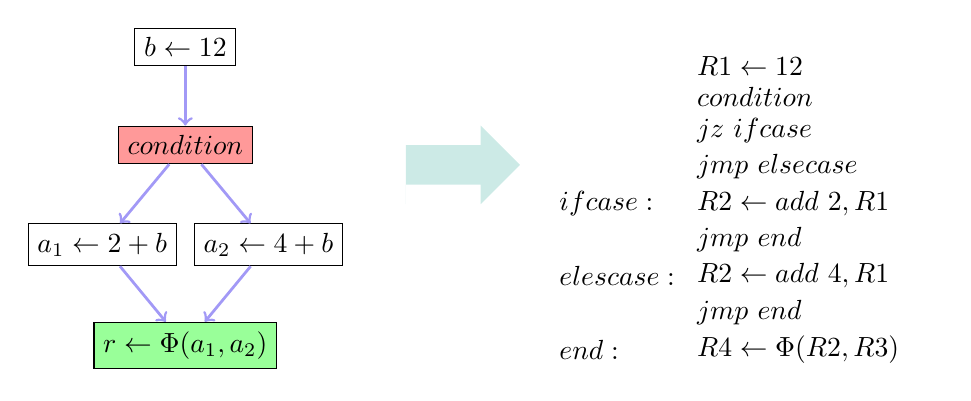
\begin{tikzpicture}[
	cfn/.style={
		draw,rectangle
	},
	cond/.style={
		fill=firmred
	},
	phi/.style={
		fill=firmgreen
	},
	cf/.style={
		color=firmblue,
		line width=1pt,
	},
	asslabel/.style={
		rectangle,
		text width=1.5cm,
		align=left
	},
	ass/.style={
		rectangle,
		text width=3cm,
		align=left
	}
]
% Graph
\node [cfn,anchor=south] at (2,2)				(ass)		{ $b \leftarrow 12$ };
\node [cfn,cond,below=0.75cm of ass]				(cond)		{ $condition$ };

\node [cfn,below left=0.75cm and -0.75cm of cond]		(left)		{ $a_1 \leftarrow 2 + b$ };
\node [cfn,below right=0.75cm and -0.75cm of cond]		(right)		{ $a_2 \leftarrow 4 + b$ };

\node [cfn,phi,below=2cm of cond]				(phi)		{ $r \leftarrow \Phi(a_1, a_2)$ };


\draw[->,cf]	(ass) to (cond);
\draw[->,cf]	(cond) to (left);
\draw[->,cf]	(cond) to (right);
\draw[->,cf]	(left) to (phi);
\draw[->,cf]	(right) to (phi);

\visible<2-> {
% Arrow
\fill [kit!20] (4.8,0.25) -- (4.8,0.5) -- (5.75,0.5) -- (5.75,0.25) -- (6.25,0.75) -- (5.75,1.25) -- (5.75,1) -- (4.8,1) -- cycle;

% Assembler
\node [ass]	at (10,2)					(aass)		{ $R1 \leftarrow 12$ };
\node [ass,below=-0.1cm of aass]				(acond)		{ $condition$ };
\node [ass,below=-0.1cm of acond]				(acondjmp1)	{ $jz\ ifcase$ };
\node [ass,below=-0.1cm of acondjmp1]				(acondjmp2)	{ $jmp\ elsecase$ };
\node [ass,below=-0.1cm of acondjmp2]				(ifass)		{ $R2 \leftarrow add\ 2, R1$ };
\node [ass,below=-0.1cm of ifass]				(ifjmp)		{ $jmp\ end$ };
\node [ass,below=-0.1cm of ifjmp]				(elseass)	{ $R2 \leftarrow add\ 4, R1$ };
\node [ass,below=-0.1cm of elseass]				(elsejmp)	{ $jmp\ end$ };
\node [ass,below=-0.1cm of elsejmp]				(endnode)	{ $R4 \leftarrow \Phi(R2, R3)$ };

\node [asslabel,left=0 of ifass]				(iflabel)	{$ifcase:$};
\node [asslabel,left=0 of elseass]				(elselabel)	{$elescase:$};
\node [asslabel,left=0 of endnode]				(endlabel)	{$end:$};
}
\end{tikzpicture}

\visible<3-> {
Challenges:
}
\begin{itemize}
\visible<3-> { \item Firm nodes not extendable in jFirm }
\visible<4-> { \item Two operand code in x86 64 assembler:\\
$R2 \leftarrow add 2, R1$ $\Rightarrow$ $mov R1, R2$, $add 2, R2$ }
\visible<5-> { \item Register allocation }
\end{itemize}
\end{frame}

\end{document}
